\chapter{Arquitetura do Sistema}\label{cap:arch_sys}

Este capítulo descreve como a ferramenta desenvolvida interage com os
\textit{softwares} em uso na competição.

Os seguintes \textit{softwares} externos são de relevância para o entendimento
da arquitetura escolhida:

\begin{itemize}
  \item ssl-vision: desenvolvido pela comunidade e de uso oficial na competição
    para processamento das imagens da câmera nas partidas e distribuição pela
    rede dos dados processados (estado do jogo);
  \item grSim: desenvolvido pela comunidade e amplamente usado pelas equipes
    para simular o ambiente das partidas, o protocolo usado para enviar o estado
    pela rede é identico ao do ssl-vision;
  \item pyroboime: também chamado de core desenvolvido pela RoboIME, atualmente provê uma camada de
    abstração sobre a comunicação com o ambiente de jogo (real ou simulado)
    incluindo redução de ruído, planejamento de trajetória e controle.
\end{itemize}

Para fins práticos o desenvolvimento ocorre com base no simulador (grSim).  O
comportamento é compatível com o real.

\section{Comunicação com Componentes Externos}

\begin{figure}[ht]
  \centering
  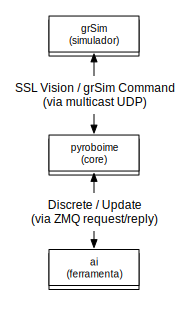
\includegraphics[height=10cm]{communication}
  \caption{Diagrama de comunicação entre os componentes.}\label{fig:arch-comm}
\end{figure}

A figura~\ref{fig:arch-comm} representa como os componentes se comunicam.  A
ferramenta se comunica apenas com o pyroboime para aproveitar todas as
funcionalidades necessárias que fogem ao escopo desse trabalho.  Por isso o foco
do desenvolvimento está concentrado em atender diretamente os objetivos.

\section{\textit{Threads} do Sistema}

\begin{figure}[ht]
  \centering
  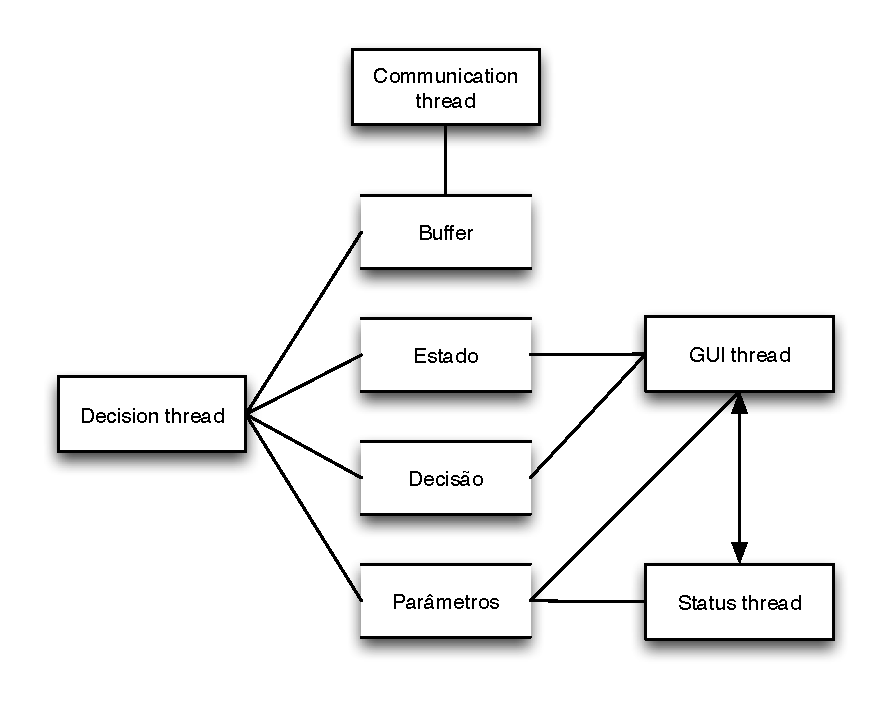
\includegraphics[height=10cm]{threads}
  \caption{Diagrama de relação entre \textit{threads} e
  dados.}\label{fig:arch-threads}
\end{figure}

A ferramenta está implementada em algumas \textit{threads} fixas de acordo com a
figura~\ref{fig:arch-threads}.  O motivo para tal distinção são os seguintes:

\begin{itemize}
  \item A interface gráfica necessita ser responsiva ao usuário.
  \item A taxa de tomada de decisão pode ser mais lenta que a taxa de
    atualização do estado, portanto a comunicação tem sua própria
    \textit{thread} que escreve e lê de um buffer compartilhado pela
    \textit{thread} de tomada de decisão.
  \item Certas informações devem ser coletadas periódicamente para atualizar
    alguns parâmetros e exibição para o usuário.
\end{itemize}


% vim: filetype=tex tw=80 et sw=2 ts=2
